
% Start preamble
\documentclass[12pt,a4paper]{article}
\usepackage{geometry}
 \geometry{
 a4paper,
 total={170mm,257mm},
 left=20mm,
 top=20mm,
 }
\usepackage[utf8]{inputenc}
\usepackage[T1]{fontenc}
\usepackage[pdftex]{graphicx}
\graphicspath{{./}}
\usepackage{enumitem}
\usepackage{pdfpages}
\usepackage{hyperref}
\usepackage{tikz}
\usepackage{attachfile}
\usepackage{epstopdf}
\usepackage{array}
\usepackage{multirow}
\usepackage{multicol}
\usepackage{float}
%\usepackage[table]{xcolor,colorbl}
\setlength{\textwidth}{17cm}
\setlength{\oddsidemargin}{-0.5cm}
\setlength{\evensidemargin}{-0.5cm}
%\setlenght{\headsep}{0cm}
\setlength\parindent{0pt}
%\setlength{\extrarowheight}{3pt}
\usepackage{listings}
%\usepackage{xcolor}

\input{arduinoLanguage.tex}
%%%%%% Counting oppgaves %%%%%%
 \newcount\questnum \questnum=0
 \def\oppgave{
            \advance\questnum by 1
	    \ifthenelse{\questnum>0\AND \questnum<9}
	    {
                \vskip 1cm
		\textbf{Oppgave}\hskip 5pt\the\questnum \hfill \hfill(6p)
		\vskip 3pt
		\hrule
	\vskip 0.5cm}
	{
                \vskip 1cm
		\textbf{Oppgave}\hskip 5pt \the\questnum \hfill \hfill(12p)
		\vskip 3pt \hrule \vskip 0.5cm }

		}

\begin{document}
\title{Prøve Grunnleggende Automasjonskunnskap}
\author{Faglærer: Fred-Olav Mosdal\\}
\maketitle
\oppgave{}%1
\vskip 2.5pt 
Hvilken strøm er størst når?
\vskip 10pt
a) $R_1=R_2=R_3$
\vskip 10pt
b) $R_2<R_1 + R_3$
\vskip 10pt
c) $R_1+R_3>R_2$
\vskip 10pt

$$\includegraphics{i04872x01.eps}$$

\vskip 5pt 

\begin{tikzpicture}
	\draw[step=0.5cm,gray!90,very thin]  grid (17,8) ;
\end{tikzpicture}
\vskip 2.5pt 

\vskip 2.5pt 
\newpage
\oppgave{}%2
\vskip 2.5pt 

Regn ut spenningsfallet og strømmen i disse to kretsene og forklar forskjellen hver motstand gjør:

$$\includegraphics[width=15.5cm]{i02666x01.eps}$$

\vskip 2.5pt 


\begin{tikzpicture}
	\draw[step=0.5cm,gray!90,very thin]  grid (17,8) ;
\end{tikzpicture}
\vskip 2.5pt 
\newpage
\oppgave{}%3
\vskip 2.5pt 
Bruk Kirchhoff's strømlov for å regne ut strømmen i $R_4$ i denne kretsen. 

$$\includegraphics[width=15.5cm]{i01161x01.eps}$$

\vskip 2.5pt 


\begin{tikzpicture}
	\draw[step=0.5cm,gray!90,very thin]  grid (17,8) ;
\end{tikzpicture}
\vskip 2.5pt 
\newpage


\oppgave{}%4
\vskip 2.5pt 

Regn ut resistansen til strekklappen i denne målebro kretsen, gitt voltmeterets indikasjon på 5.6mV (A er positiv og B er negativ).

$$\includegraphics[width=15.5cm]{i00854x01.eps}$$

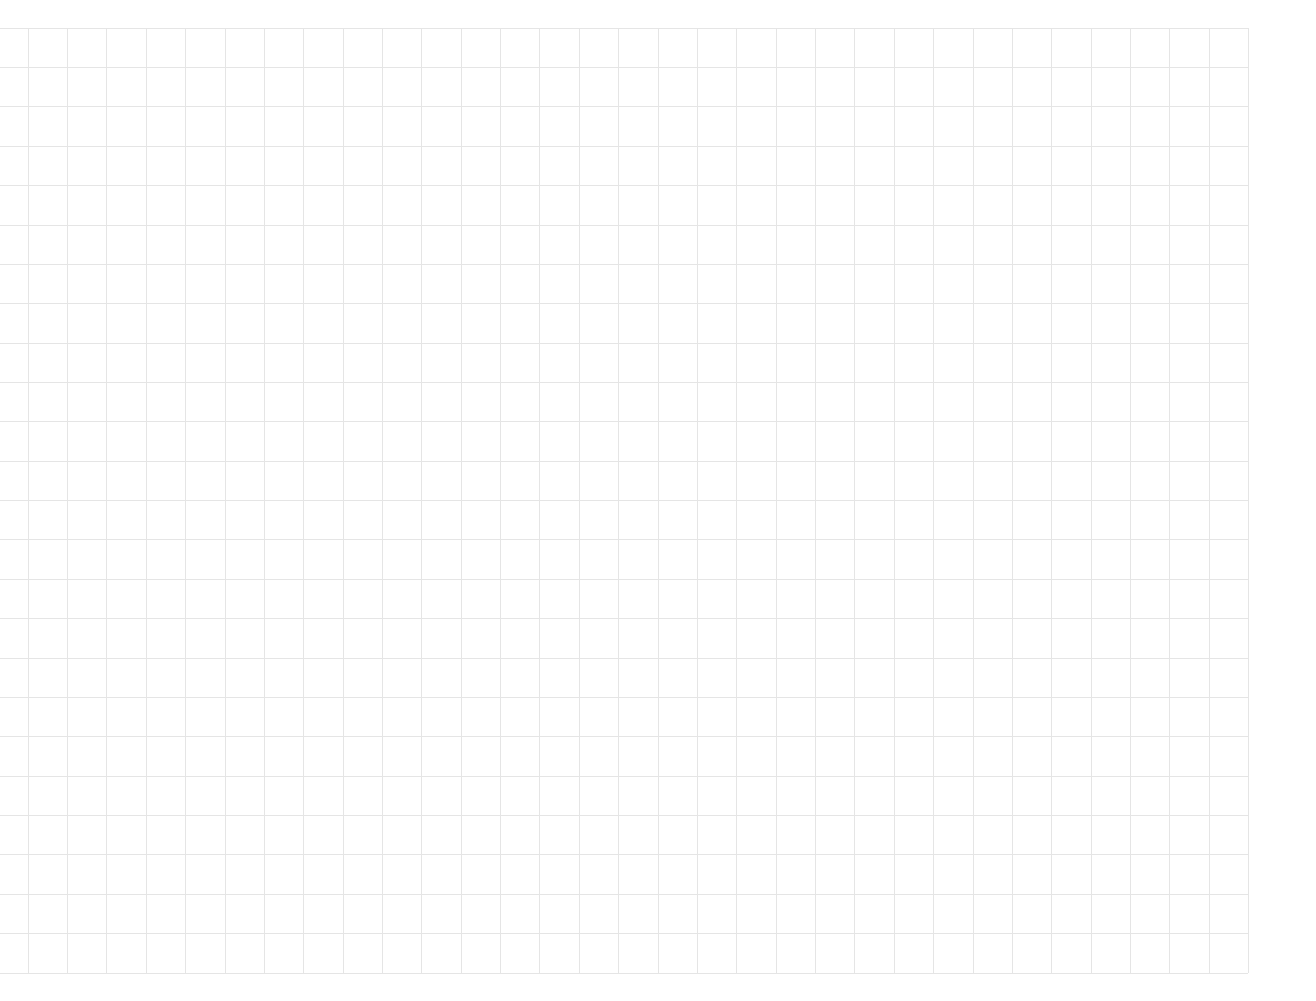
\begin{tikzpicture}
	\draw[step=0.5cm,gray!20,very thin]  grid (16,12) ;
\end{tikzpicture}
$R_{strain}$ = \underbar{\hskip 50pt}

\vskip 2.5pt 


\begin{tikzpicture}
	\draw[step=0.5cm,gray!90,very thin]  grid (17,8) ;
\end{tikzpicture}
\vskip 2.5pt 
\newpage
\oppgave{}%5
\vskip 2.5pt 
Finn spenningen i forhold til jord for hvert av punktene \textbf{A} og \textbf{B} i kretsen under. 
Kretsen kan være i 4 ulike tilstander: begger brytere av, bryter A på og B Av, Bryter A av og B på og begge på. Du må finne spenningene for alle tilstandene. 

$$\includegraphics[width=15.5cm]{i01133x01.eps}$$

% No blank lines allowed between lines of an \halign structure!
% I use comments (%) instead, so that TeX doesn't choke.

$$\vbox{\offinterlineskip
\halign{\strut
\vrule \quad\hfil # \ \hfil & 
\vrule \quad\hfil # \ \hfil & 
\vrule \quad\hfil # \ \hfil & 
\vrule \quad\hfil # \ \hfil & 
\vrule \quad\hfil # \ \hfil \vrule \cr
\noalign{\hrule}
%
% First row
Voltage & Both loads off & Load 1 on (only) & Load 2 on (only) & Both loads on \cr
%
\noalign{\hrule}
%
% Second row
$U_A$ &  &  &  &  \cr
%
\noalign{\hrule}
%
% Third row
$U_B$ &  &  &  &  \cr
%
\noalign{\hrule}
} % End of \halign 
}$$ % End of \vbox

\vskip 2.5pt 


\begin{tikzpicture}
	\draw[step=0.5cm,gray!90,very thin]  grid (17,8) ;
\end{tikzpicture}
\vskip 2.5pt 
\newpage
\oppgave{}%6
\vskip 2.5pt 

Regn ut motstanden mellom punkt \textbf{A} og \textbf{B} i de ulike kretsene nedenfor. 

$$\includegraphics[width=15.5cm]{i01165x01.eps}$$
\vskip 2.5pt 


\begin{tikzpicture}
	\draw[step=0.5cm,gray!90,very thin]  grid (17,8) ;
\end{tikzpicture}
\vskip 2.5pt 
\newpage
\oppgave{}%7
\vskip 2.5pt 

Regn ut spenningsfallet over $R_2$:

$$\includegraphics[width=15.5cm]{i01166x01.eps}$$
\vskip 2.5pt 


\begin{tikzpicture}
	\draw[step=0.5cm,gray!90,very thin]  grid (17,8) ;
\end{tikzpicture}
\vskip 2.5pt 
\newpage
\oppgave{}%8
\vskip 2.5pt 

Calculate the following circuit parameters, assuming the transmitter has been calibrated to a range of 25 to 150 inches of water column (direct-acting, 4 to 20 mA output).  Be sure to show all your calculations!

$$\includegraphics[width=15.5cm]{aBasicx08.eps}$$
\begin{itemize}
\item{} $I$ = \underbar{\hskip 50pt} mA
\vskip 10pt
\item{} $V_{C}$ = \underbar{\hskip 50pt} V 
\vskip 10pt
\item{} $V_{BC}$ = \underbar{\hskip 50pt} V 
\vskip 10pt
\item{} $V_{B}$ = \underbar{\hskip 50pt} V 
\end{itemize}
\vskip 2.5pt 


\begin{tikzpicture}
	\draw[step=0.5cm,gray!90,very thin]  grid (17,8) ;
\end{tikzpicture}
\vskip 2.5pt 
\oppgave{}%9
\vskip 2.5pt 

Her vises to transmittere som er koblet til en regulator med to innganger. Transmitterene får forsysningspenning fra strømsløyfen(4-20mA). Til utgangen på regulatoren er det koblet en I/P konverter som brukes til å styre en pneumatisk reguleringsventil. Inngangen på regulatoren har et område på 1-5V, ikke 4-20mA. 

$$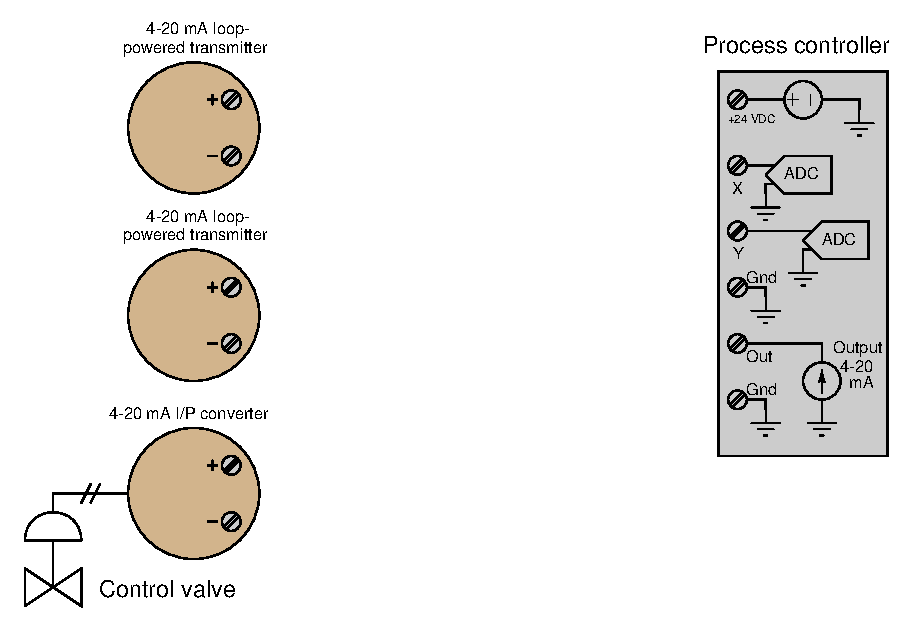
\includegraphics[width=15.5cm]{i02273x01.eps}$$

Vis hvordan feltutstyret skal kobles til regulatoren, inkluder plassering av motstander for konvertere strømsignal til spenningssignal som regulatorens ADC kan lese. Bruk skjermet kabel og vis hvordan denne skal jordes. 


\vskip 2.5pt 


\begin{tikzpicture}
	\draw[step=0.5cm,gray!90,very thin]  grid (17,8) ;
\end{tikzpicture}
\vskip 2.5pt 
\newpage
\end{document}
